\documentclass{scrartcl}

\usepackage[latin1]{inputenc}
\usepackage{amsmath}
\usepackage{shortvrb}
\setlength\parindent{0pt}
\setlength\parskip{10pt}



\usepackage{tikz}
\usetikzlibrary{arrows}
\usetikzlibrary{shadows}
\usetikzlibrary{shapes}
\usetikzlibrary{backgrounds}
\usetikzlibrary{positioning}

\def\tikzname{Ti\emph{k}Z}

\begin{document}
\MakeShortVerb{\|}

\section{Nodes}
%==============
\subsection{Introduction}
%------------------------
A simple |\node| example:\\
\tikz \node [circle, draw, red] {hello};

A node with semicircle shape and a \LaTeX\ math environment:\\
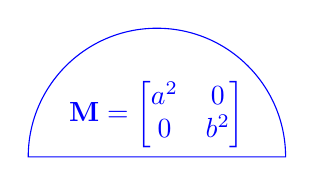
\begin{tikzpicture}
  \node [semicircle, draw, blue] {
      $\mathbf{M} = \begin{bmatrix}
        a^2 & 0 \\
        0 & b^2 \\
      \end{bmatrix}$
    };
\end{tikzpicture}

A node showing some graphic options and containing a minipage:\\
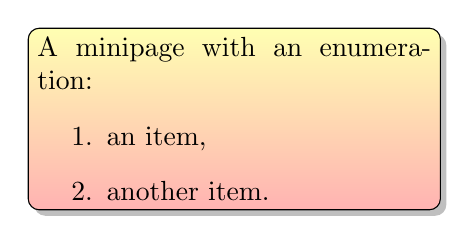
\begin{tikzpicture}
  \node [rectangle, rounded corners, draw, drop shadow, shade, top color=yellow!30, bottom color=red!30] {
    \begin{minipage}{5cm}%
      A minipage with an enumeration:
      \begin{enumerate}
        \item an item,
        \item another item.
      \end{enumerate}
    \end{minipage}
  };
\end{tikzpicture}



\subsection{Placing Nodes}
%-------------------------
Defining a style for |packet| nodes:\\
\tikzset{packet/.style={rectangle, draw, very thick,
           minimum size=8mm, rounded corners=1mm,
           fill=red!30!orange!30, drop shadow}}
\tikz \node[packet] (p1) at (0,0) {$p_1$};

Placing nodes using absolute coordinates:\\
\begin{tikzpicture}[scale=1.2]
  \path [draw, gray!50, very thin] (0,0) grid (5,2);
  \node[packet] (p1) at (0,1.5) {$p_1$};
  \node[packet] (p2) at (1,1.5) {$p_2$};
  \node[packet] (p3) at (2,1.5) {$p_3$};
  \node[packet] (pn) at (5,1.5) {$p_n$};
  \node[packet] (p1') at (0,0) {$p_1$};
  \node[packet] (p2') at (1,0) {$p_2$};
  \node[packet] (p3') at (2,0) {$p_3$};
\end{tikzpicture}

\newpage
Placing nodes using relative positioning:\\
\begin{tikzpicture}[node distance=2mm]
  \node[packet] (p1)                    {$p_1$};
  \node[packet] (p2)  [right=of p1]     {$p_2$};
  \node[packet] (p3)  [right=of p2]     {$p_3$};
  \node[packet] (pn)  [right=3cm of p3] {$p_n$};
  \node[packet] (p1') [below=1cm of p1] {$p_1$};
  \node[packet] (p2') [right=of p1']    {$p_2$};
  \node[packet] (p3') [right=of p2']    {$p_3$};
  \node (f)           [left=of p1]      {$f$:};
  \node (prefix)      [left=of p1']     {$\operatorname{prefix}(f,3)$:};
\end{tikzpicture}

Anchors 1:\\
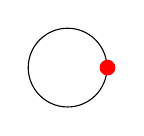
\begin{tikzpicture}
  \node [circle, draw, minimum size=1cm] (c) {};
  \path [fill=red] (c.east) circle (1mm);
\end{tikzpicture}

Anchors 2:\\
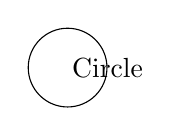
\begin{tikzpicture}
  \node [circle, draw, minimum size=1cm] (c) {};
  \node at (c.east) {Circle};
\end{tikzpicture}

Anchors 2:\\
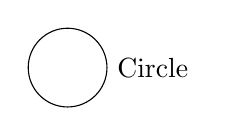
\begin{tikzpicture}
  \node [circle, draw, minimum size=1cm] (c) {};
  \node [anchor=west] at (c.east) {Circle};
\end{tikzpicture}

Anchors of the rectangle shape (from the \tikzname\ manual):\\
\tikzset{
  shape example/.style={
    color=black!30,
    draw,
    fill=yellow!30,
    line width=.3cm,
    inner xsep=1.7cm,
    inner ysep=0.5cm}
}
\begin{tikzpicture}
  \Huge
  \node[name=s,shape=rectangle,shape example] {Rectangle\vrule width 1pt height 2cm};
  \foreach \anchor/\placement in
      {north west/above left, north/above, north east/above right,
       west/left, center/above, east/right,
       south west/below left, south/below, south east/below right,
       mid west/left, mid/above, mid east/right,
       base west/left, base/below, base east/right,
       text/left, 10/right, 130/above}
      \draw[shift=(s.\anchor)] plot[mark=x] coordinates{(0,0)} node[\placement] {\scriptsize\texttt{(s.\anchor)}};
\end{tikzpicture}


\subsection{Connecting Nodes}
%----------------------------
The |to| path-operation:\\
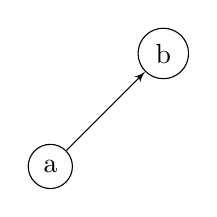
\begin{tikzpicture}[>=latex']
  \node [circle, draw] (a) {a};
  \node [circle, draw] (b) [above right=of a] {b};
  \draw [->] (a) to (b);
\end{tikzpicture}

\newpage
The |to| path-operation with the |bend left| option:\\
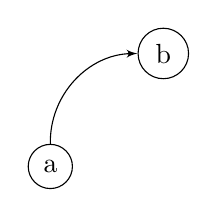
\begin{tikzpicture}[>=latex']
  \node [circle, draw] (a) {a};
  \node [circle, draw] (b) [above right=of a] {b};
  \draw [->] (a) to [bend left=45] (b);
\end{tikzpicture}

The |to| path-operation with the |out| and |in| option:\\
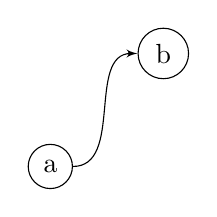
\begin{tikzpicture}[>=latex']
  \node [circle, draw] (a) {a};
  \node [circle, draw] (b) [above right=of a] {b};
  \draw [->] (a) to [out=0, in=180] (b);
\end{tikzpicture}

Labeling Connections 1 (|auto|):\\
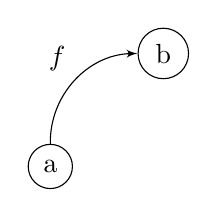
\begin{tikzpicture}[>=latex']
  \node [circle, draw] (a) {a};
  \node [circle, draw] (b) [above right=of a] {b};
  \draw [->] (a) to [bend left=45] node [auto] {$f$} (b);
\end{tikzpicture}

Labeling Connections 2 (|swap|):\\
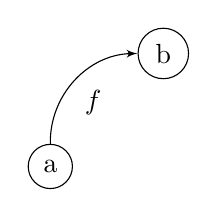
\begin{tikzpicture}[>=latex']
  \node [circle, draw] (a) {a};
  \node [circle, draw] (b) [above right=of a] {b};
  \draw [->] (a) to [bend left=45] node [auto, swap] {$f$} (b);
\end{tikzpicture}

Labeling Connections 3 (|very near start|):\\
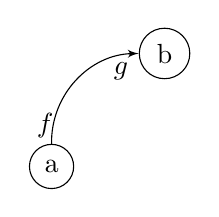
\begin{tikzpicture}[>=latex']
  \node [circle, draw] (a) {a};
  \node [circle, draw] (b) [above right=of a] {b};
  \draw [->] (a) to [bend left=45]
          node [xshift=-1mm, very near start] {$f$}
          node [yshift=-2mm, very near end] {$g$} (b);
\end{tikzpicture}

The |edge| path-operation:\\
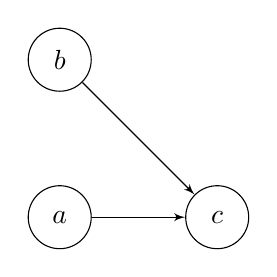
\begin{tikzpicture}[>=latex', node distance=2cm,
                    state/.style = {circle, draw, minimum size=8mm},
                    transition from/.style = {<-}]
  \node [state] (a) {$a$};
  \node [state] (b) [above of=a] {$b$};
  \node [state] (c) [right of=a] {$c$}
    edge [transition from] (a)
    edge [transition from] (b);
\end{tikzpicture}

\newpage

\begin{tikzpicture}[node distance=2mm]
  \node[packet] (p1)                    {$p_1$};
  \node[packet] (p2)  [right=of p1]     {$p_2$};
  \node[packet] (p3)  [right=of p2]     {$p_3$};
  \node[packet] (pn)  [right=3cm of p3] {$p_n$};
  \node[packet] (p1') [below=1cm of p1] {$p_1$};
  \node[packet] (p2') [right=of p1']    {$p_2$};
  \node[packet] (p3') [right=of p2']    {$p_3$};
  \node (f)           [left=of p1]      {$f$:};
  \node (prefix)      [left=of p1']     {$\operatorname{prefix}(f,3)$:};
  \draw [ultra thick, dotted, shorten >=3mm, shorten <=3mm] (p3) to (pn);
\end{tikzpicture}

\newpage
Flow prefix picture:\\
\begin{tikzpicture}[node distance=2mm]
 \draw (0,10) -- (20,10)--(20,3)--cycle;
\end{tikzpicture}

%With great power comes great responsibility:\\
%\tikz \node [minimum size = 4cm, rectangle, dashed, ultra thick, color=red!80!yellow, rounded corners, draw, drop shadow, shade, top color=red!50!blue, bottom color=green] {\Huge *The End.*};
\newpage
\begin{tikzpicture}
\node [mybox] (box){%
    \begin{minipage}{1.00\textwidth}
        \begin{enumerate}
			\item Diffusion.
			\item Permeation.
			\item Sorption( Adsorption) \& Desorption.
	   	 	\item Evaporation.
			\item Interaction of charged , neutral particle and photon with surface.
			\item Chemical Reactions at Solid Surfaces.
			\item Gassing and Degassing of the Surface.
	
	\end{enumerate}
    \end{minipage}
};
\node[fancytitle, right=10pt] at (box.north west) {A fancy title};
%\node[fancytitle, rounded corners] at (box.east) {$\clubsuit$};
\end{tikzpicture}%


\end{document}

% vim::set expandtab tabstop=4 softtabstop=2 shiftwidth=2:
